\section{Background}
We analyze the requirements of provisioning timely and high-quality video in variable network conditions compared with the traditional streaming framework, and propose to customize the whole broadcaster-side RTMP protocol stack for the goal. Due to the constraints of existing practical architecture and deployment policy, applying none-RTMP-based solutions is not compatible with the other existing part of the whole system (e.g., the CDN in the middle).

\begin{figure}[t]
\centerline{\includegraphics[width=0.9\columnwidth]{fig/architecture.pdf}}
\vspace{-0.08in}
\caption{Architecture of personalized live streaming.}
\vspace{-0.1in}
\label{fig:architecture}
\end{figure}
\textbf{Video streaming architecture.}
Figure~\ref{fig:architecture} shows the (simplified) common architecture 
of popular personalized live streaming platforms. When live streaming 
starts, the broadcaster uploads the live video to an edge server using 
RTMP protocols, from which the video is forwarded to many CDN edge servers 
as other content (e.g., web) using traditional overlay distribution 
protocols. Finally, each viewer streams the video from a nearby edge
server using HTTP-based streaming protocols (i.e., DASH).

\textbf{Personalized live streaming.}
Personalized live streaming uprises recently, it evolves from traditional live streaming (e.g., ESPN's sports broadcast
and CNN's scheduled programs). Both kinds of streaming share the goal to distribute video content to a large audience at a low cost and  rely on existing CDN infrastructure to distribute video content to viewers through HTTP-based streaming protocols. However, personalized live streaming distinguishes itself from 
other live streaming settings in two key aspects, which is oftern overlooked right now.

{\em 1. Individual mobile users as broadcasters}
Traditional live streaming (e.g., ESPN) uses a dedicated
over-provisioned connection (usually direct cable or an exclusive
satellite channel) to stream high-resolution raw video
content from a camera to a special content management
server, which then transcodes the original video into video chunks.
In contrast, the content source in personalized video
streaming is often mobile users who upload the live video
through a wireless connection shared with many other users. Due to the broadcaster motion and complicated wireless signal strength in the environment, personalized live streaming broadcasters may meet with more variable network conditions.

{\em 2. Broadcaster-viewer interactivity.}
Moreover, ensuring low end-to-end streaming delay is critical
in personalized live streaming for broadcasters
to interact with viewers, while viewers in traditional sports live
events watch the video only passively.
For instance, the broadcaster wants to show her gratitude 
instantaneously if she gets a gift from a viewer.
Therefore, the streaming delay ideally should be no more than
several seconds, which is much less than traditional live
streaming which typically tolerates around 10 seconds of end-to-end 
delay (e.g., sports events).

%\subsection{Broadcaster streaming protocols}
\textbf{Design requirements.} These differences lead to three requirements on the broadcaster streaming protocol design.\\
{\em 1. High video quality.} Video quality includes metrics about a video itself, including bitrate, frame-per-second, resolutions, etc. The broadcaster must provide videos with the highest possible quality to the CDN so that the downstream viewers can get satisfactory QoE.\\
{\em 2. Agile adaptation.} The streaming protocol must be sufficiently adaptive to quickly react the bandwidth fluctuations in wireless networks.\\
{\em 3. Timeliness.} The streaming protocol must ensure the streaming delay between the broadcaster and viewers is minimized
or at least bounded.

\textbf{Constraints for practical deployment.}
For practical reasons, RTMP has become the de-facto
broadcaster streaming protocol in most of today's platforms,
including Facebook Live, Twitch, Periscope, Panda Tv,
Douyu, and so forth.
RTMP is flexible enough to potentially meet
the three aforementioned requirements.
For instance, it offers several tunable parameters for
the broadcaster to adjust the video quality, including
frames per second (FPS), buffer size, and frame dropping
policy.
In theory, the frame-dropping policy could
strike a dynamic balance between quality and timeliness
in the presence of throughput fluctuation
(e.g.,~\cite{huang2003adaptive,krasic2003quality,singh2004dynamic}).
Nonetheless, as we will show in the next section,
both commercial implementations of RTMP and
the up-to-date open source RTMP implementation suffer from similar quality degradation.

Alternative HTTP-based broadcaster streaming protocols have also
been studied, including using DASH~\cite{pires2014dash}, HTTP POST~\cite{seo2012experimental},
and adaptively switching between them~\cite{wilk2016leveraging}.
While switching from RTMP to HTTP-based protocols might
achieve better video quality, it requires costly
changes to client-side software and cannot react to wireless
fluctuation in a timely manner due to chunking overheads
(each chunk is at least of
several seconds).

\iffalse
There are a few tunable parameters for the broadcaster to adjust the video quality. They are frames per second (FPS), resolution, and bitrate. Then the streaming software uses H.264 to compress the video and push it to the RTMP server. H.264 uses two mechanisms to compress video. First, instead of streaming raw frames, it sends a few keyframes and sends the delta between the keyframes and the non-keyframes. Second, if the result frames still exceed the pre-configured bitrate, a filter would be used to generate ``big pixels'' in the video pictures, which reduce frame size but sacrifices video quality.


\textbf{Requirements of personalized live streaming.}
Compared with VoD and traditional living streaming, the personalized live streaming
has two unique requirements, bad network resistance and low streaming delay.

In VoD, the video is ready on servers for the audience to fetch; in traditional living streaming, the video source side usually reserve network bandwidth from ISP to upload real-time video from its source to servers, and similarly the audience fetch the video from a nearby server. While in personalized live streaming, the video generation environment may be complicated (e.g., our door activities, unstable radio access network), thus there is no guarantee for the network condition to upload videos to servers. Thus, the personalized video should be resistant to bad network conditions (e.g., low throughput, network jitters).

Another important feature in personalized video streaming is that it has systems (e.g., chatting, gifting) for the broadcaster and the audience to interact with each other. In this scenario, video delay is not tolerable; that is, personalized live streaming has more requirements on timeliness that traditional live streaming and VoD. For example, the broadcaster may want to thank the audience instantaneously if he/she is given gifts; in game streaming, without instantaneous feedback from the audience, the broadcaster may make frustrating mistakes.
\fi


\iffalse
In this section, we describe the general architecture of the interactive live video streaming system.
\subsection{Interactive Live Video Streaming System}
Interactive live video streaming system is composed of three major components: (1) Streamer side; (2) CDN servers; (3) Viewer side, as shown in figure\ref{fig_architecture}. Each streamer is equipped with a software, like OBS, twitch tools, that captures the camera or screen in real-time and encodes into H.264 format, then transmitted to the video platform through RTMP. The video platform distributes the streaming over CDN servers, and the viewers request the streaming from one edge server.

\begin{figure}[t]
\centering
\includegraphics[width=0.9\columnwidth]{architecture.pdf}
\vspace{-0.08in}
\caption{Interactive Live Video Streaming System}
\vspace{-0.1in}
\label{fig_architecture}
\end{figure}

While in live video streaming systems, frames are produced by a video frame generation thread and consumed by a frame sending thread, which is a typical producer-consumer model. Frames in the buffer are organized naturally in a temporal order. We propose smarter buffer management mechanisms, where we have timeliness as the first-priority goal and meanwhile increase the most number of decodable frames.

Compared with traditional live video streaming, there are two fundamental differences: 1) the streamers are often mobile devices in diverse and varying wireless environments, which indicates no performance guarantee on network connections, 2) instantaneous interaction (e.g., chatting) between the streamer and the audience requires strict low end-to-end latency (several seconds), which is much shorter than traditional live streaming (tens of seconds).

Each component will introduce delay into the system, and a long latency will obviously affect the interactivity. To avoid queuing latency in live video streaming systems, the streamer side and the viewer side usually adopt shallow buffers or queues to improve timeliness (e.g., the 0.7-second buffer in OBS streamer application).
With shallow buffer and varying wireless environments, the smooth watching experience becomes a challenge.

\subsection{Timeliness Control}
In practical scenarios where the underline network fails to provide stable bandwidth (e.g., mobile live streaming), the streamer side usually chooses to drop frames to guarantee the timeliness.
There exists three kinds of frames, `I', `P', `B', in H.264 format. `I' frames are independent, `P' frames depend on previous `I` or `P' frames. `B' frames depend on previous and later `I', or `P' frames. Missing higher priority frames will lead to decoding error to lower priority frames.

Due to the frame dependency of decode,
\fi 
